\documentclass{beamer}
\usepackage[utf8]{inputenc}
\usepackage[frenchb]{babel}
\usepackage{lmodern}
\usepackage{amssymb}
\usepackage[T1]{fontenc}
\usepackage[lined,boxed,french,onelanguage]{algorithm2e}

\title{Oral du projet de Programmation Objet}
\author{Maxime Arthaud \and Martin Carton \and Korantin Auguste}

\date{13 mai 2013}

\begin{document}
  \begin{frame}
    \titlepage
  \end{frame}

  \begin{frame}{Introduction}
    \begin{itemize}
      \item Un format de fichier pour pour pouvoir écrire des scènes à la main,
        dans une interface graphique ou automatiquement.

      \item
        Deux programmes:
        \begin{itemize}
          \item Une interface graphique pour éditer un fichier représentant une
            scène.
          \item Un programme en ligne de commande pour générer une image à
            partir d'un fichier de scène.
        \end{itemize}
    \end{itemize}
  \end{frame}

  \begin{frame}{Interface utilisateur}
    \centerline{
      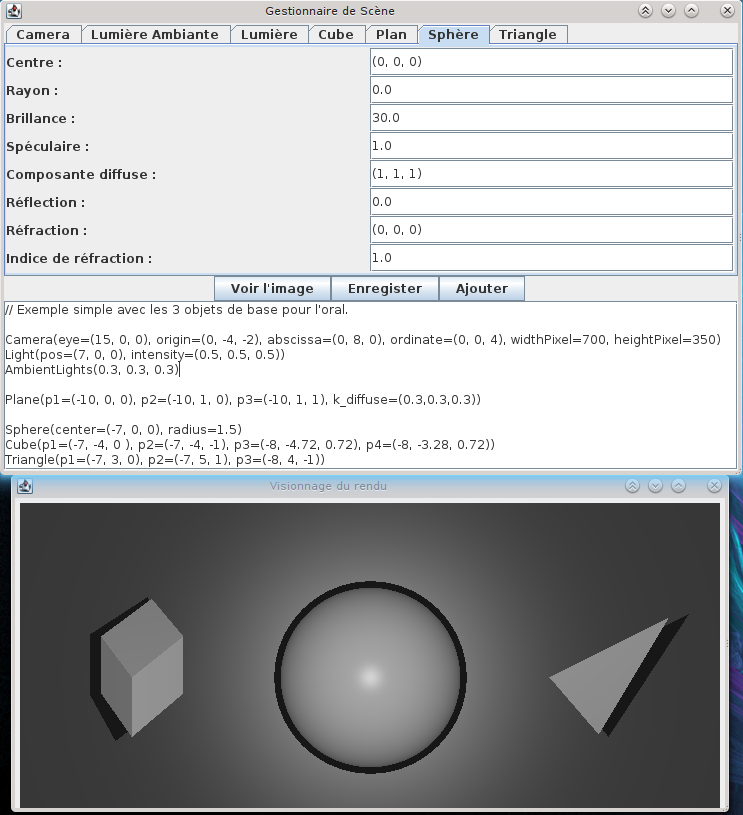
\includegraphics[height=0.8\paperheight, keepaspectratio=true]
      {screen2.png}
    }
  \end{frame}

  \begin{frame}{Exemple de rendu plus complexe}
    \centerline{
      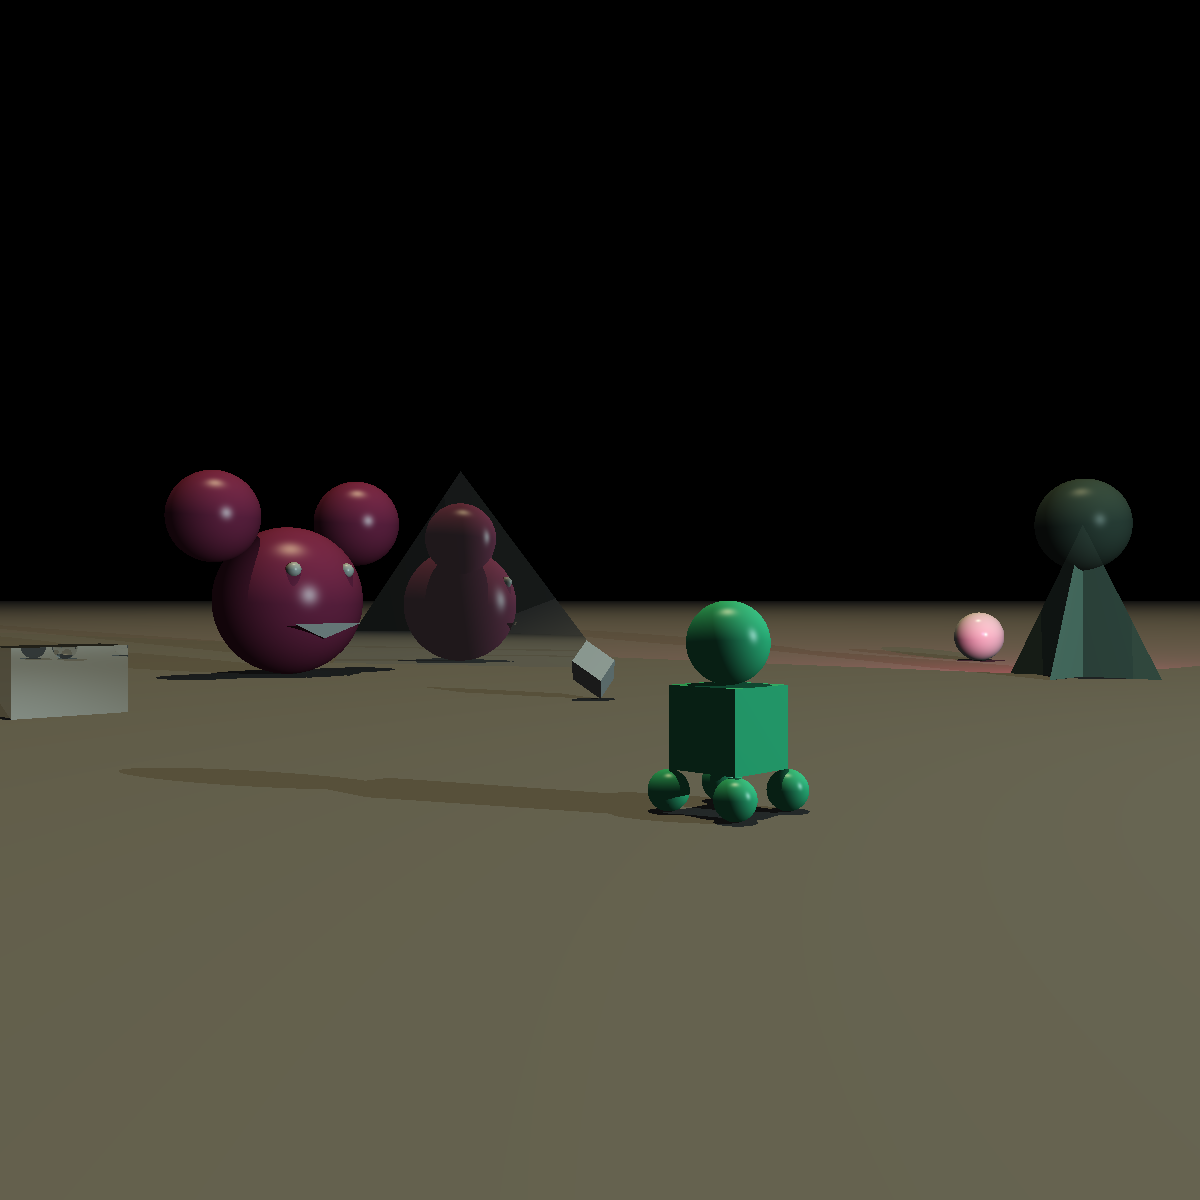
\includegraphics[width=\textwidth, height=0.8\paperheight,
      keepaspectratio=true]{0377.png}
    }
  \end{frame}

  \begin{frame}{Exemple de rendu plus complexe, autre point de vue}
    \centerline{
      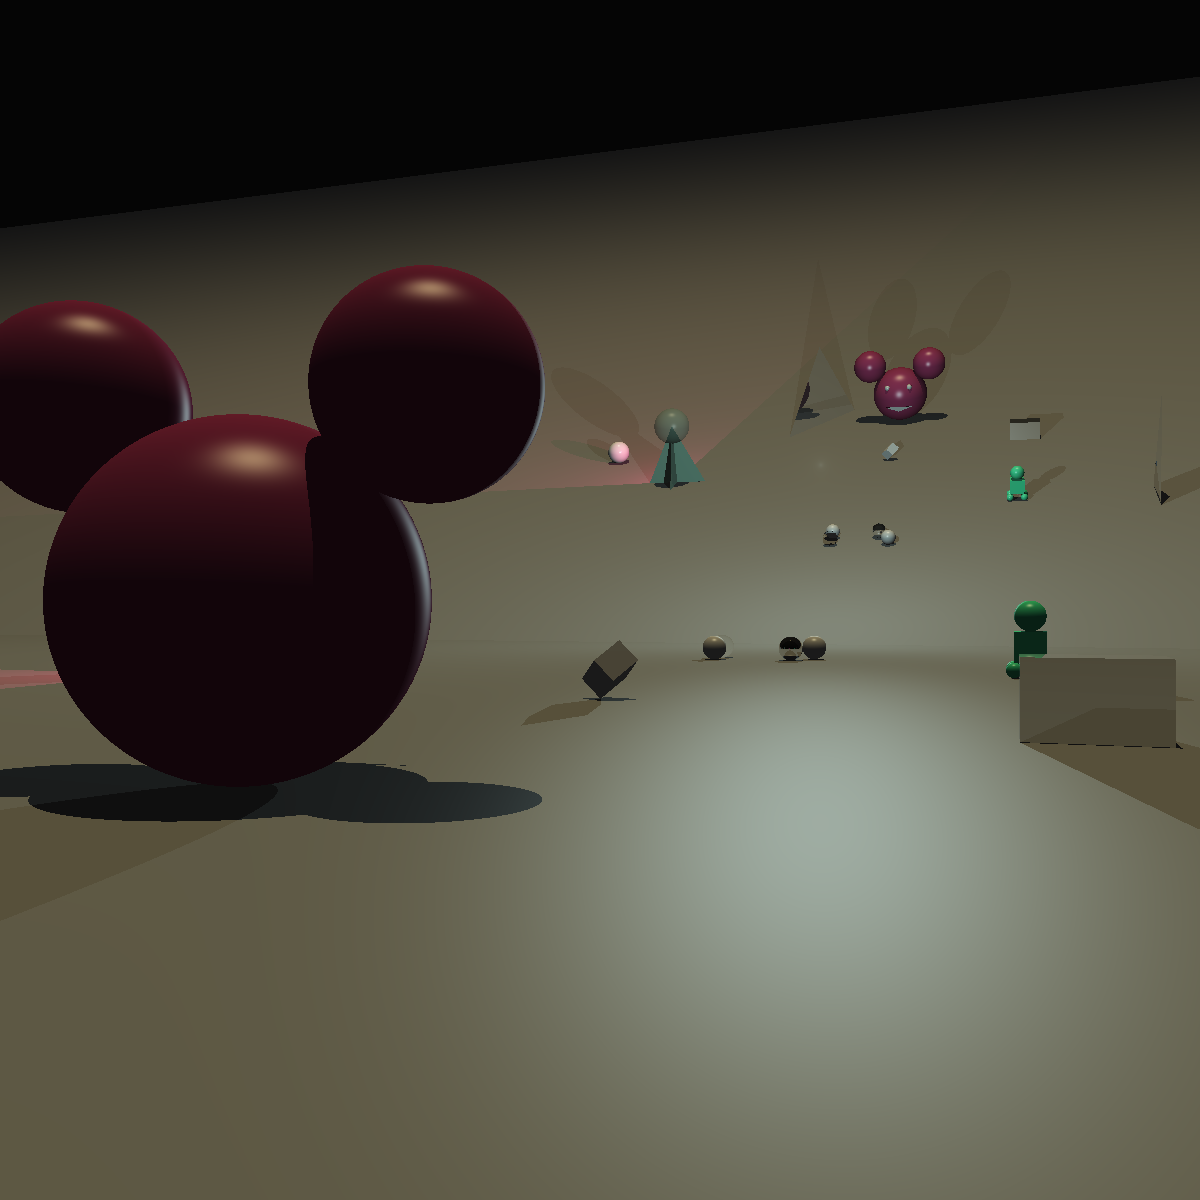
\includegraphics[width=\textwidth, height=0.8\paperheight,
      keepaspectratio=true]{0699.png}
    }
  \end{frame}
\end{document}
